\pdfminorversion=7
\documentclass[english, usepdftitle=false, svgnames, color="table, fixpdftex, fixinclude, xcdraw", t]{beamer}

\usepackage{lode-i18n}
\usepackage{lode-srccode}
\usepackage{lode-imacid}
\usepackage{lode-pdf}

\usepackage{common-table}
\usepackage{tabularx}
\usepackage{multirow}

\usepackage{animate}
\usepackage{movie15}

\usepackage{inputx}
\inputpaths{../CommonAssets/}

\graphicspath{{../CommonAssets/}}


\title{Software testing}
\subtitle{Functional testing}
\author[]{%
Marco Aurelio Graciotto Silva\inst{1}, \\\and
}

\newcommand{\numberofinstitutes}{1}
\institute[UTFPR]
{
	\inst{1}%
	Federal University of Technology -- Parana (UTFPR)\\
	Campo Mourao, PR, Brazil
}
% \institute[ICMC]
% {
% 	\inst{2}%
% 	University of Sao Paulo (USP)\\
% 	Sao Carlos, SP, Brazil
% }


\date[]{February 2014}

% \logopicture{icmc-qualipso-inf}
% \logopicture{icmc-qualipso-inf}


\begin{document}

\frontmatter{}
../CommonAssets/preamble.tex


\mainmatter{}
\part{Functional testing}
\section{Functional testing}
\begin{frame}[c,parent={cmap:software-testing}, hasprev=false, hasnext=false]
\frametitle{Functional testing}
\label{cmap:functional-testing}

\insertcmap{Courses-SoftwareTesting-FunctionalTesting}
\end{frame}



\begin{frame}[parent={cmap:functional-testing}, hasprev=false, hasnext=true]
\frametitle{Functional testing}
\label{concept:functional-testing}

\begin{block:concept}{Functional testing}
Functional testing is a technique in which testing is based solely on the
requirements and specifications.
\end{block:concept}

\begin{block:fact}{Black-box testing}
	\centering
	\includegraphics[width=\textwidth]{resources/Functional testing/Black box testing (no requirements)}
\end{block:fact}
\end{frame}


\begin{frame}[hasprev=true, hasnext=true]
\frametitle{Functional testing}
\label{concept:black-box}

\begin{columns}[t]
\column{.6\textwidth}
\begin{block:fact}{Black box}
\begin{itemize}
	\item Functional testing considers the product under test as a box:
	\begin{itemize}
		\item of which are only known its input and outputs;

		\item which may only be visualized from its exterior.
	\end{itemize}

	\item It requires no knowledge of the internal paths, structure, or
	implementation of the software.
\end{itemize}
\end{block:fact}

\column{.4\textwidth}
\includegraphics[scale=.3]{resources/Functional testing/Black box}
\end{columns}
\end{frame}



\begin{frame}
\frametitle{Functional testing}
\framesubtitle{Test phases}

\begin{block:fact}{Test phases}
\begin{itemize}
	\item Functional testing can be applied at any of the test phases.

	\item Functional testing approach remains the same regardless of the size
	and the input/output complexity of the software (unit, module, subsystem)
	under testing.
\end{itemize}
\end{block:fact}


\begin{block:fact}{Test phases}
\begin{itemize}
	\item Actually, software testing of big software pieces forces the tester
	to use functional testing as there are simply too many paths through the
	software to apply other test techniques.
\end{itemize}
\end{block:fact}
\end{frame}


\begin{frame}
\frametitle{Functional testing}
\framesubtitle{Limitations}

\begin{block:fact}{Limitations}
\begin{itemize}
	\item Functional testing depends upon good software requirements
	specification.

	\item Functional testing is not suitable for testing complex processing
	that requires simple input data.
\end{itemize}
\end{block:fact}
\end{frame}



\begin{frame}[hasprev=true, hasnext=false]
\frametitle{Functional testing}

\begin{block:procedure}{Basic steps for functional testing}
\begin{enumerate}
	\item The software requirements are analyzed.
	\begin{itemize}
		\item Valid inputs are chosen based on the software requirements
		to determine that the software processes them correctly.

		\item Invalid inputs must also be chosen to verify that the software
		detects them and handles them properly.
	\end{itemize}

	\item Expected outputs for those inputs are determined.

	\item Test cases are constructed with the selected inputs.

	\item The test cases are run.

	\item Actual outputs are compared with the expected outputs.

	\item A determination is made as to the proper functioning of the software.
\end{enumerate}
\end{block:procedure}
\end{frame}


\subsection{Equivalence partition}
\begin{frame}[ parent={concept:functional-testing}, hasprev=false, hasnext=true]
\frametitle{Equivalence partition}
\label{concept:equivalence-partition}

\begin{block:concept}{Equivalence partition}
Equivalence partition divides the input conditions, identified from the
product, into valid and invalid equivalence classes.
\end{block:concept}

\begin{block:fact}{Rationale}
\begin{itemize}
	\item It considers each element of a given equivalence class as equivalent.
	\begin{itemize}
		\item If a certain element of a given equivalence class is able to
		detect a fault, every other element of that same equivalence class
		is also able to detect the same fault.
	\end{itemize}

	\item Thus, the correct establishment of the partitions is essential for
	this criterion.
	\begin{itemize}
		\item However, requirements often lacks details to perform this
		correctly.
	\end{itemize}
\end{itemize}
\end{block:fact}
\end{frame}



\begin{frame}[hasnext=true, hasprev=true]
\frametitle{Equivalence partition}

\begin{block:fact}{Equivalence partition}
\begin{itemize}
	\item Equivalence partition requires a test set to cover:
	\begin{itemize}
		\item the valid equivalence classes (\textbf{one} test case can cover
		\textbf{more than one} valid classes),

		\item and \textbf{one} test case to cover \textbf{each} of the invalid
		equivalence classes.
	\end{itemize}
\end{itemize}
\end{block:fact}

\begin{block:fact}{Why one test case for each invalid class?}
\begin{itemize}
	\item Invalid classes are in general related to a special implementation
	code to produce differentiated error messages.

	\item Combining several invalid classes in a single test case may conceal
	such error messages.
\end{itemize}
\end{block:fact}
\end{frame}


\begin{frame}
\frametitle{Equivalence partition}
\label{procedure:equivalence-partition}

\begin{block:fact}{Two steps}
The equivalence partition is organized in two phases:
\begin{itemize}
	\item identification of equivalence classes,
	\item definition of test cases for the classes identified.
\end{itemize}
\end{block:fact}


\begin{block:procedure}{Procedure}
\begin{enumerate}
	\item Identify equivalence classes.
	\begin{enumerate}
		\item Identify the relevant input conditions.
		\item Partition each condition in two or more groups.
	\end{enumerate}

	\item Define the test cases to cover those classes.
	\begin{enumerate}
		\item Assign a number for every class.
		\item Define test cases to cover the greatest number of valid classes
		as possible, until every valid class is covered.
		\item For every invalid class, design an specific test case.
	\end{enumerate}
\end{enumerate}
\end{block:procedure}

\hfill
\refie{example:equivalence-partition}{\beamerbutton{Example}}
\end{frame}


\begin{frame}
\frametitle{Equivalence partition}
\framesubtitle{Partition guidelines}

\begin{block:fact}{Partitioning guidelines}
\begin{itemize}
	\item The identification of equivalence partitions is, largely, a
	heuristic process.

	\item For some situations, there are some well established guidelines
	that can be used.
\end{itemize}
\end{block:fact}

\begin{block:fact}{Tipical situations}
\begin{itemize}
	\item Constants
	\item Enumerations
	\item Sequences
	\item Ranges
\end{itemize}
\end{block:fact}
\end{frame}


\begin{frame}
\frametitle{Equivalence partition}
\framesubtitle{Partition guidelines}

\begin{block:fact}{Constants}
\begin{itemize}
	\item If an input condition specified a single restriction or constant
	value for the value, there will be two classes:
	\begin{itemize}
		\item One valid for the value with the constant.
		\item One invalid for the value without the constant.
	\end{itemize}
\end{itemize}
\end{block:fact}

\begin{block}{Example}
\begin{itemize}
	\item The requirement states that ``the first character of the identifier
	must be a letter''.

	\item There are two equivalence classes:
	\begin{itemize}
		\item Valid class: the first letter of the identifier is a letter.
		\item Invalid class: the first letter of the identifier is not a
		letter.
	\end{itemize}
\end{itemize}
\end{block}
\end{frame}



\begin{frame}
\frametitle{Equivalence partition}
\framesubtitle{Partition guidelines}

\begin{block:fact}{Enumeration}
\begin{itemize}
	\item If an input condition specifies a set of N input values and there is
	a reason to believe that the program handles each one differently, there
	will be N + 1 classes:
	\begin{itemize}
		\item N valid classes for each acceptable input value.
		\item One invalid for a value not in the enumeration.
	\end{itemize}
\end{itemize}
\end{block:fact}

\begin{block}{Example}
\begin{itemize}
	\item The requirement states that ``the type of the vehicle must be BUS,
	TRUCK, CAB, FOOT''.

	\item There are five equivalence classes:
	\begin{itemize}
		\item Valid classes: one class for each vehicle type (BUS, TRUCK,
		CAB, FOOT).
		\item Invalid class: one class for a vehicle not present in the
		enumeration (AIRCRAFT).
	\end{itemize}
\end{itemize}
\end{block}
\end{frame}



\begin{frame}
\frametitle{Equivalence partition}
\framesubtitle{Partition guidelines}

\begin{block:fact}{Sequence}
\begin{itemize}
	\item If the input condition specifies a sequence of values, there are three
	partitions:
	\begin{itemize}
		\item One valid, for the values within the sequence.

		\item Two invalid, for values lower than the bottom value and greater
		than top value of the sequence.
		range.
	\end{itemize}
\end{itemize}
\end{block:fact}


\begin{block}{Example}
\begin{itemize}
	\item The requirement states that ``one throught six owners can be listed
	for the automobile''.

	\item There are three equivalence classes:
	\begin{itemize}
		\item Valid class: list of owners with one to six names.
		\item Invalid classes:
		\begin{itemize}
			\item empty owner list,
			\item owner list with more than six names.
		\end{itemize}
	\end{itemize}
\end{itemize}
\end{block}
\end{frame}



\begin{frame}
\frametitle{Equivalence partition}
\framesubtitle{Partition guidelines}

\begin{block:fact}{Range}
\begin{itemize}
	\item If the input condition specifies a range of values, there are three
	partitions:
	\begin{itemize}
		\item One valid, for the values within the range.

		\item Two invalid, for values lower than the bottom value and greater
		than top value of the range.
		range.
	\end{itemize}
\end{itemize}
\end{block:fact}


\begin{block}{Example}
\begin{itemize}
	\item The requirement states that ``the item count can be from 1 to 999''.

	\item There are three equivalence classes:
	\begin{itemize}
		\item Valid class: item count between 1 and 999 (including the number
		1 and 999).
		\item Invalid classes:
		\begin{itemize}
			\item item count with a value less than 1,
			\item item count with a value greater than 999.
		\end{itemize}
	\end{itemize}
\end{itemize}
\end{block}
\end{frame}



\begin{frame}
\frametitle{Equivalence partition}
\framesubtitle{Limitations}

\begin{block:fact}{Limitations}
\begin{itemize}
	\item The equivalence partition assumption is too strong in practice.
	\begin{itemize}
		\item It is quite common to have data-sensible faults which require a
		specific value inside an equivalence class in order to be detected.
	\end{itemize}

	\item Equivalence partition does not explore input condition combinations.
\end{itemize}
\end{block:fact}
\end{frame}

\subsection{Boundary value analysis}
\begin{frame}[hasprev=false, hasnext=true, parent={concept:functional-testing}]
\frametitle{Boundary value analysis}

\begin{block:fact}{}
\begin{itemize}
	\item Experience shows that test cases that explore \textbf{boundary
	conditions} have a higher payout than test cases that do
	not~\cite[p. 59]{myers:2004}.

	\item Hence it would be interesting to have a test criterion that
	exploited such situations.
\end{itemize}
\end{block:fact}
\end{frame}


\begin{frame}[hasprev=true, hasnext=true]
\frametitle{Boundary value analysis}
\label{concept:boundary-value-analysis}

\begin{block:concept}{Boundary value analysis}
Boundary value analysis requires that test cases be selected based on the
boundaries of each equivalence class.
\end{block:concept}

\begin{block:fact}{Boundary value analysis and equivalent partition}
\begin{itemize}
	\item Boundary value analysis is complementary to equivalent partition.

	\item It explores boundary conditions, such as the same, above and below
	limits in the equivalence class.
\end{itemize}
\end{block:fact}
\end{frame}


\begin{frame}
\frametitle{Boundary value analysis}
\framesubtitle{Boundary for a range}

\begin{block:fact}{Boundary for a range}
\begin{itemize}
	\item The input for a test case for an input which boundary conditions
	establish a range of values must be:
	\begin{itemize}
		\item in the limits of the range,
		\item above and below the limits.
	\end{itemize}
\end{itemize}
\end{block:fact}
\end{frame}


\begin{frame}
\frametitle{Boundary value analysis}
\framesubtitle{Boundary for a range}

\begin{block}{Example of boundaries for a range}
\begin{itemize}
	\item The requirement states that ``the item count can be from 1 to 999''.

	\item There are three equivalence classes:
	\begin{itemize}
		\item Valid class: item count between 1 and 999 (including the number
		1 and 999).
		\item Invalid classes:
		\begin{itemize}
			\item item count with a value less than 1
			\item item count with a value greater than 999.
		\end{itemize}
	\end{itemize}

	\item The values to be tested are:
	\begin{itemize}
		\item 0 (just below/out the range)
		\item 1 (just in the range considering the lower limit)
		\item 999 (just in the range considering the upper limit)
		\item 1000 (just above/out the range)
	\end{itemize}
\end{itemize}
\end{block}
\end{frame}



\begin{frame}
\frametitle{Boundary value analysis}
\framesubtitle{Boundary for a sequence}

\begin{block:fact}{Boundary for a sequence}
\begin{itemize}
	\item The input of a test case for an input which boundary conditions
	establish a sequence of values must be:
	\begin{itemize}
		\item in the limit,
		\item and one unit below and above the limit.
	\end{itemize}
\end{itemize}
\end{block:fact}
\end{frame}


\begin{frame}
\frametitle{Boundary value analysis}
\framesubtitle{Boundary for a sequence}

\begin{block}{Example}
\begin{itemize}
	\item The requirement states that ``one throught six owners can be listed
	for the automobile''.

	\item There are three equivalence classes:
	\begin{itemize}
		\item Valid class: list of owners with one to six names.
		\item Invalid classes:
		\begin{itemize}
			\item empty owner list,
			\item owner list with more than six names.
		\end{itemize}
	\end{itemize}

		\item The values to be tested are:
	\begin{itemize}
		\item 0 (one unit below the limit)
		\item 1 (just in the limit considering the lower limit)
		\item 5 (just in the limit considering the upper limit)
		\item 7 (one unit above the limit)
	\end{itemize}
\end{itemize}
\end{block}
\end{frame}


\begin{frame}[hasprev=true, hasnext=false]
\frametitle{Boundary value analysis}
\framesubtitle{Limitations}

\begin{block:fact}{Limitations}
\begin{itemize}
	\item Boundary value analysis does not explore input condition combinations.
\end{itemize}
\end{block:fact}
\end{frame}

\subsection{Cause effect graph}
\begin{frame}[hasprev=false, hasnext=true]
\frametitle{Cause-effect graph example}
\label{example:cause-effect-graph}

\begin{block}{Specification}
The character in column 1 must be an ``A'' or a ``B''. The character is column
2 must be a digit. In this situation, the file must be updated. If the first
character is incorrect, the message X12 must be issued. If the second character
is not a digit, the message X13 must be issued.
\end{block}

\begin{block}{Causes}
\begin{itemize}
	\item \textbf{(1)} Character in column 1 is ``A''.
	\item \textbf{(2)} Character in column 1 is ``B''.
	\item \textbf{(3)} Character in column 2 is a digit.
\end{itemize}
\end{block}

\begin{block}{Effects}
\begin{itemize}
	\item \textbf{(70)} file is updated.
	\item \textbf{(71)} message X12 is issued.
	\item \textbf{(72)} message X13 is issued.
\end{itemize}
\end{block}
\end{frame}



\begin{frame}[hasprev=true, hasnext=true]
\frametitle{Cause-effect graph example}

\begin{block}{Cause-effect graph}
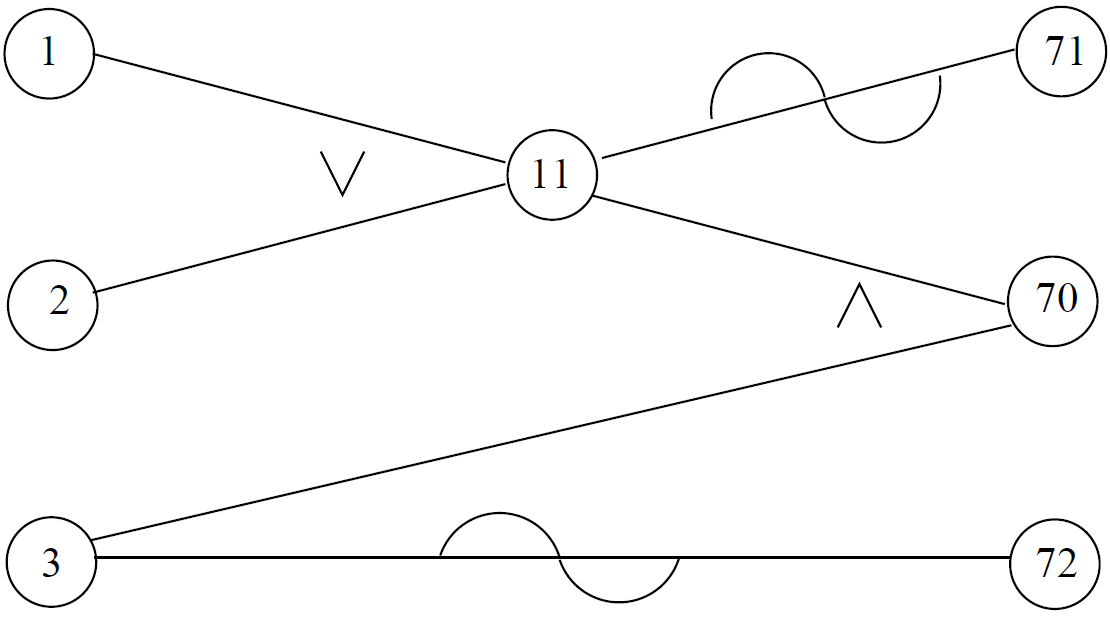
\includegraphics[width=\textwidth]{aux/examples/cause-effect-graph/Cause-effect graph example}
\end{block}

\end{frame}


\begin{frame}
\frametitle{Cause-effect graph example}

\begin{block}{Cause-effect graph (with constraints)}
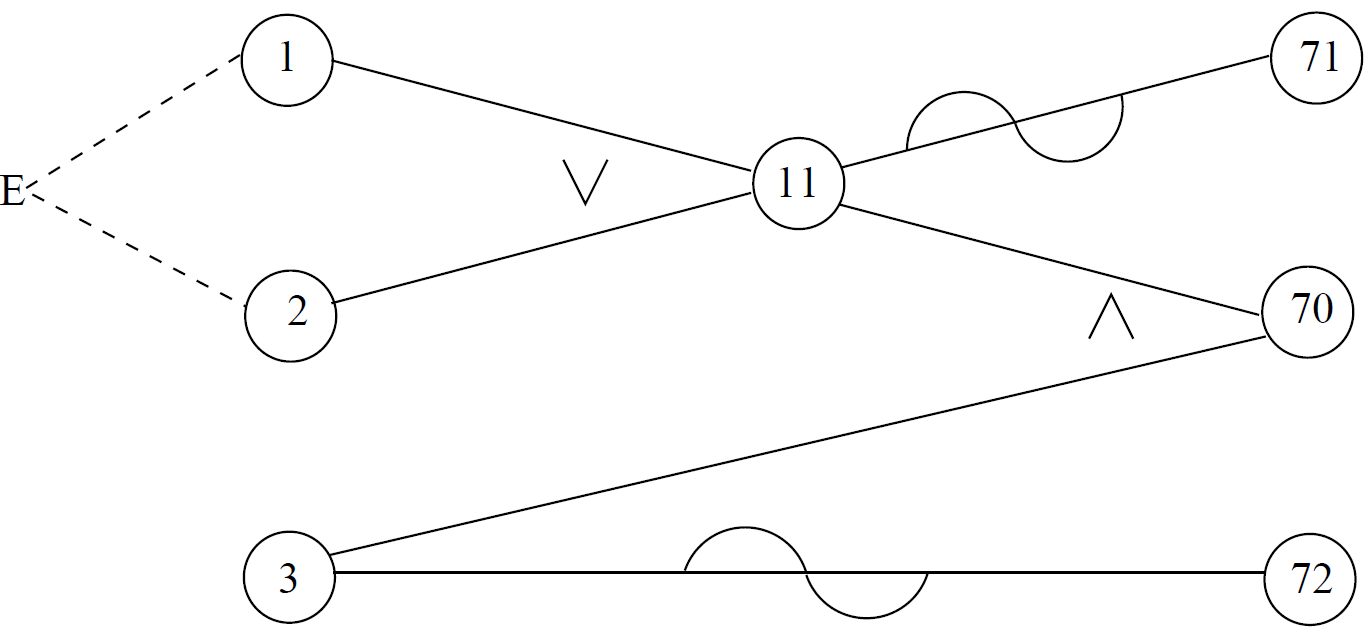
\includegraphics[width=\textwidth]{aux/examples/cause-effect-graph/Cause-effect graph example (with constraints)}
\end{block}
\end{frame}



\begin{frame}[hasprev=true, hasnext=false]
\frametitle{Cause-effect graph example}

\begin{block}{Digital circuit}
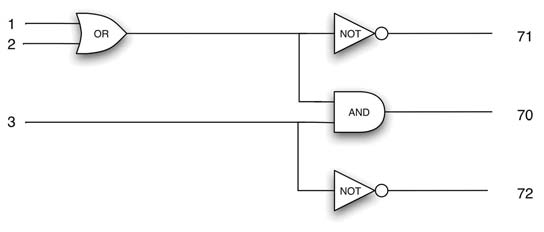
\includegraphics[width=\textwidth]{aux/examples/cause-effect-graph/Cause-effect graph to digital circuit example}
\end{block}

\end{frame}


\backmatter{}
\part{References and credits}
\part{References}
\section*{References}


\begin{frame}[label=references, allowframebreaks]{\refname}
\bibliographystyle{abnt-num}
\bibliography{root}
\end{frame}

\part{Acknowledgement}
\section*{Acknowledgement}


\begin{frame}[c,label=credits]
\frametitle{Credits}

\begin{itemize}
	\item Reviewers:
	\begin{itemize}
		\item Marcio Eduardo Delamaro
	\end{itemize}
\end{itemize}
\end{frame}


\part{Instructional elements}
\section{Examples}


% Structural software testing
%
\part{Structural software testing}
\subsection{Control flow graph}
\insertexample{identifier-cfg}{concept:cfg-graph-elements}

\subsection{Definition-use graph}
\insertexample{program-graph}{concept:definition-use-graph}

\subsection{Identifier definition-use graph}
\insertexample{identifier-dug}{concept:definition-use-graph}


% Path
%
\part{Path}
\subsection{Infeasible path}
\insertexample{identifier-infeasible-path}{concept:infeasible-path}

\subsection{Complete path}
\insertexample{identifier-complete-path}{concept:complete-path}

\subsection{Definition-clear paths example}
\insertexample{identifier-def-clear-path}{concept:definition-clear-path}


% Control flow test criterion
%
\part{Control-flow based testing}
\subsection{All-nodes}
\insertexample{all-nodes}{concept:all-nodes}

\subsection{All-paths infeasibility}
\insertexample{all-paths}{concept:all-paths}


% Complexity-based test criterion
%
\part{Complexity-flow based testing}
\subsection{McCabe example}
\insertexample{mccabe}{procedure:mccabe-criterion}


% Data flow test criterion
%
\part{Data-flow based testing}
\subsection{All-Uses for Identifier}
\insertexample{identifier-all-uses}{concept:all-uses}

\subsection{All-Pot-Uses for Identifier}
\insertexample{identifier-all-pot-uses}{concept:all-pot-uses}

\section{Exercises}



\end{document}
